\section{Sequence Diagrams}

\todo{Add diagram covering the MouseClickListeners up to onEmptyVertexClick() or onVisualVertexClick().}

\begin{figure}[h]
	\centering
	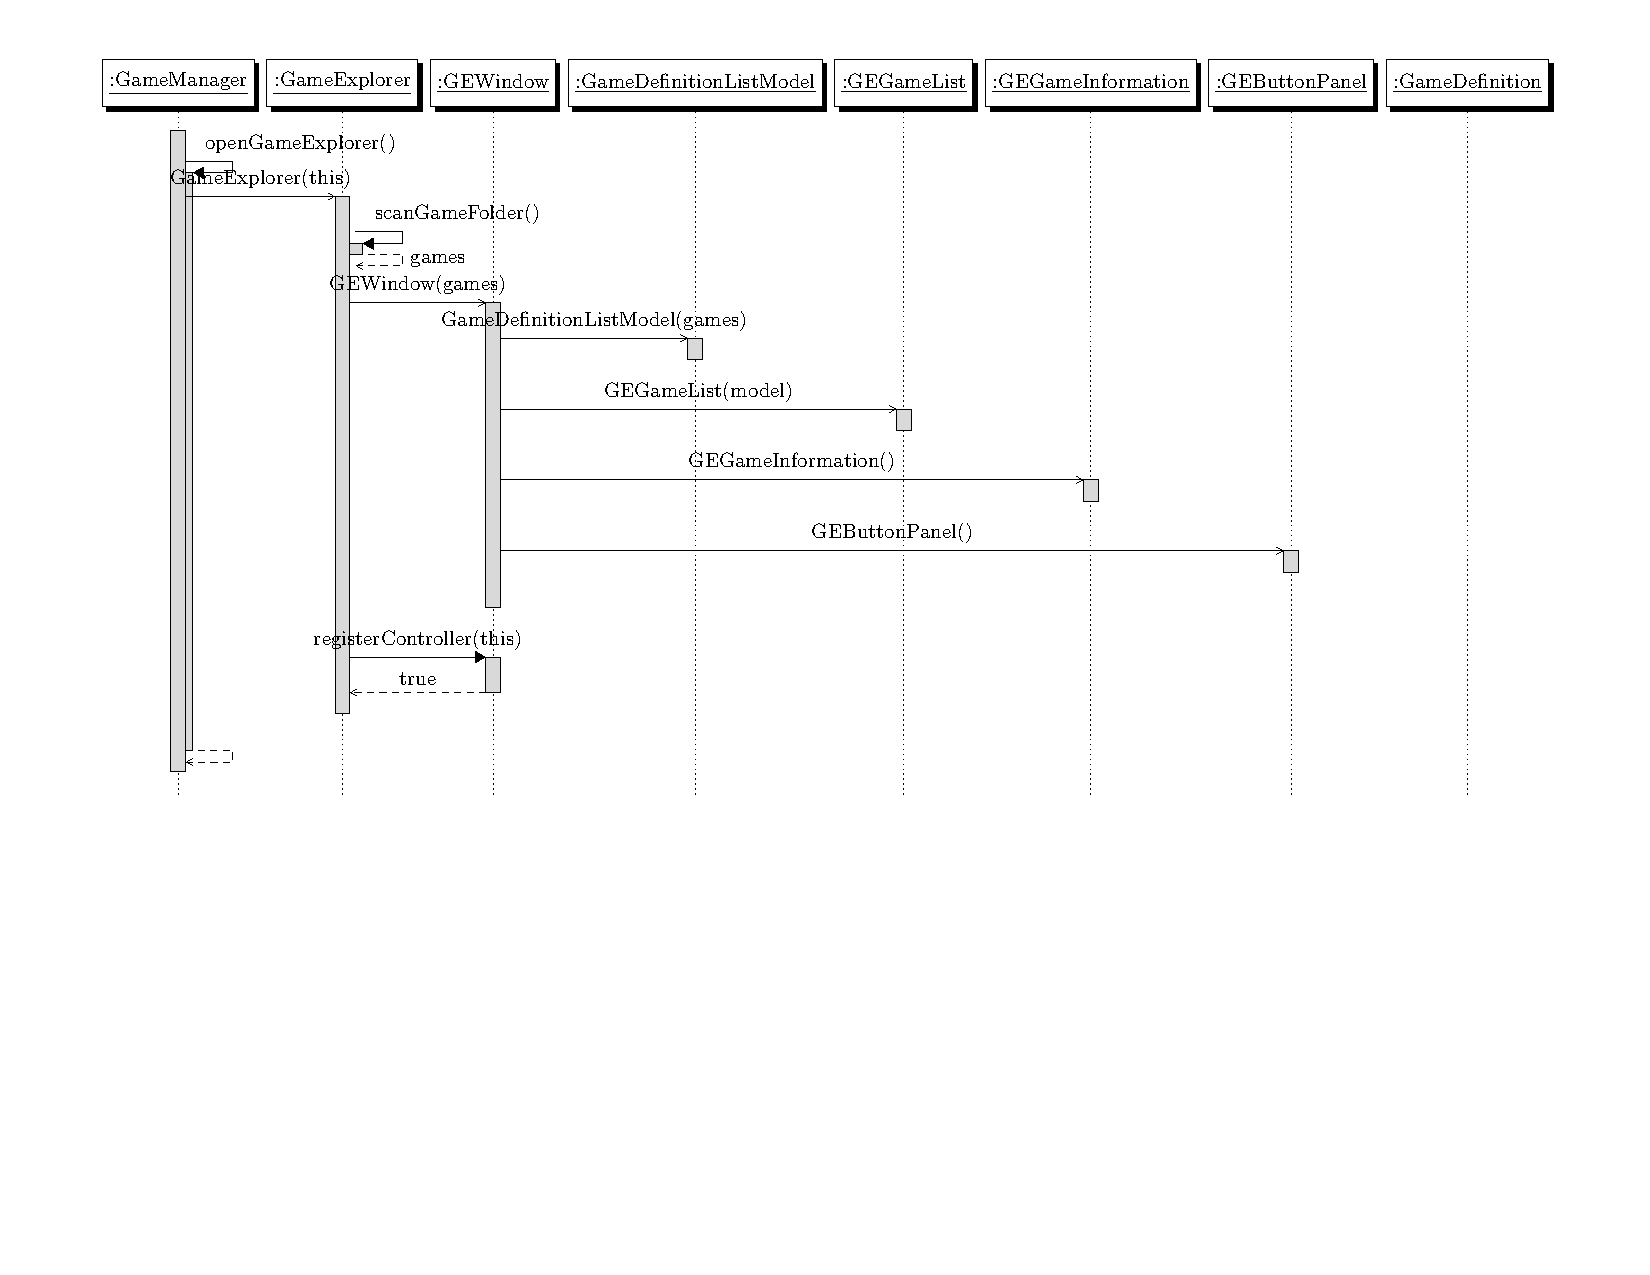
\includegraphics[page=1,angle=90,height=0.72\textheight,keepaspectratio]{seqGameExplorer.pdf}
	\caption{Sequence diagram showing the process of initializing the \gameexplorer.}
	\label{img:seqGameExplorer}
\end{figure}

\begin{figure}[h]
	\centering
	\includegraphics[page=2,angle=90,width=1\textwidth]{seqGameExplorer.pdf}
	\caption{Sequence diagram showing the process of selecting a game with an initialized \gameexplorer.}
	\label{img:seqGameExplorer}
\end{figure}

\begin{figure}[h]
	\centering
	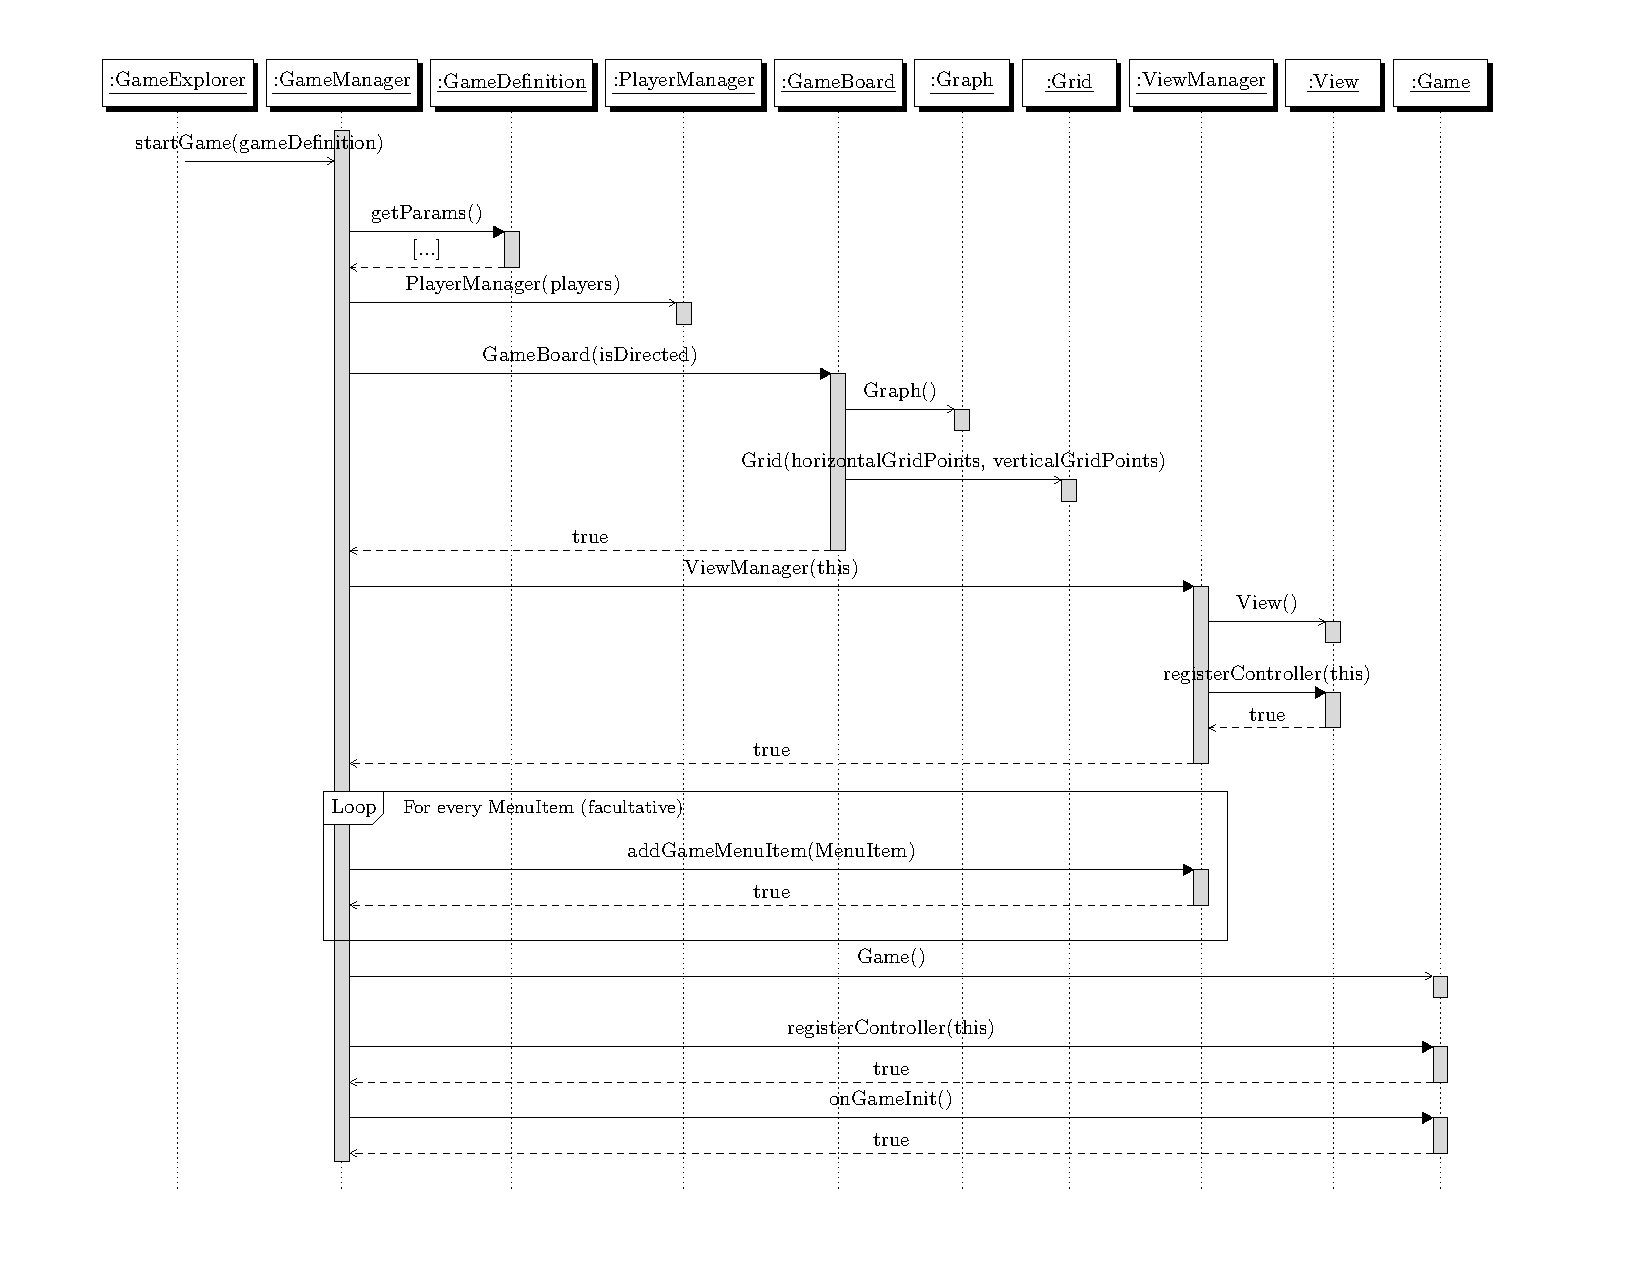
\includegraphics[angle=90,width=1\textwidth]{seqGameInitialization.pdf}
	\caption{Sequence diagram showing the process of a game's initialization.}
	\label{img:seqGameInitialization}
\end{figure}

\begin{figure}[h]
	\centering
	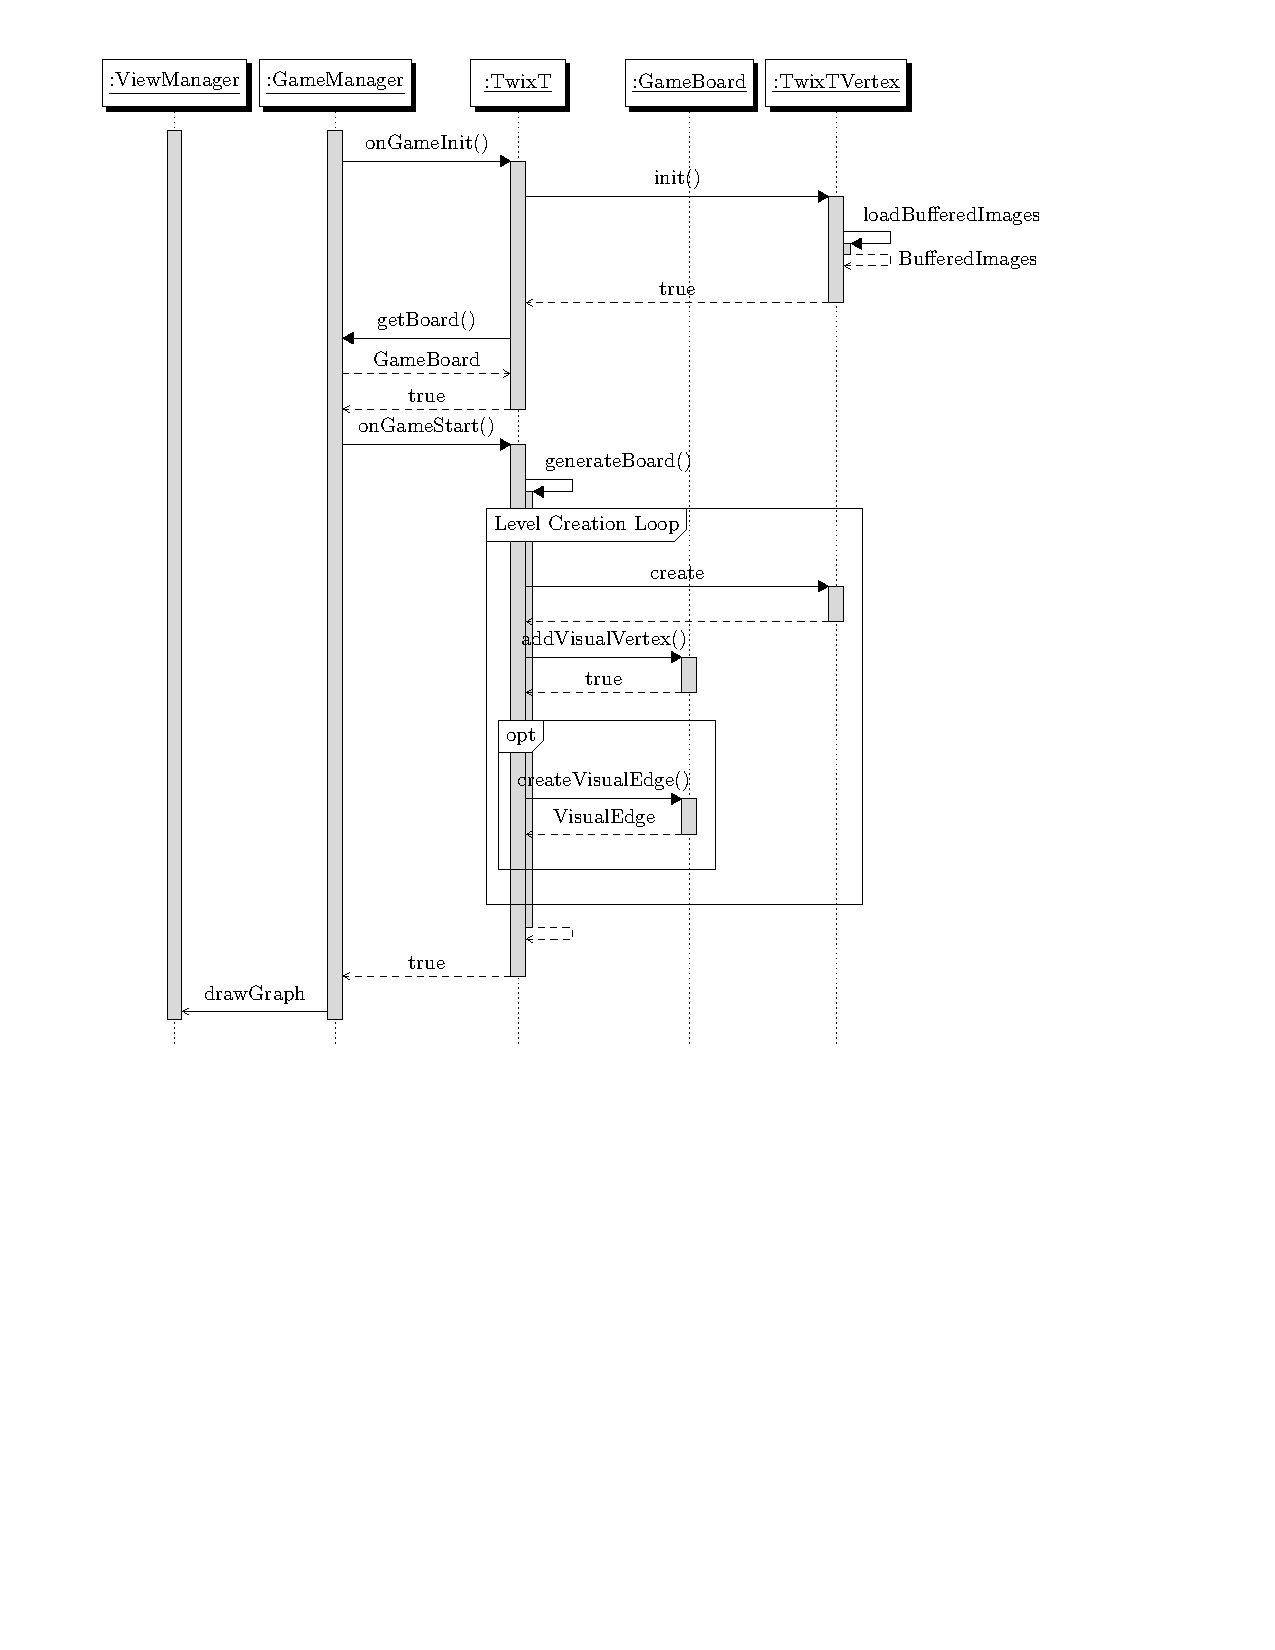
\includegraphics[width=1\textwidth]{seqTwixTStartup.pdf}
	\caption{Sequence diagram showing the process of initializing a new \twixt game.}
	\label{img:seqTwixTStartup}
\end{figure}

\begin{figure}[h]
	\centering
	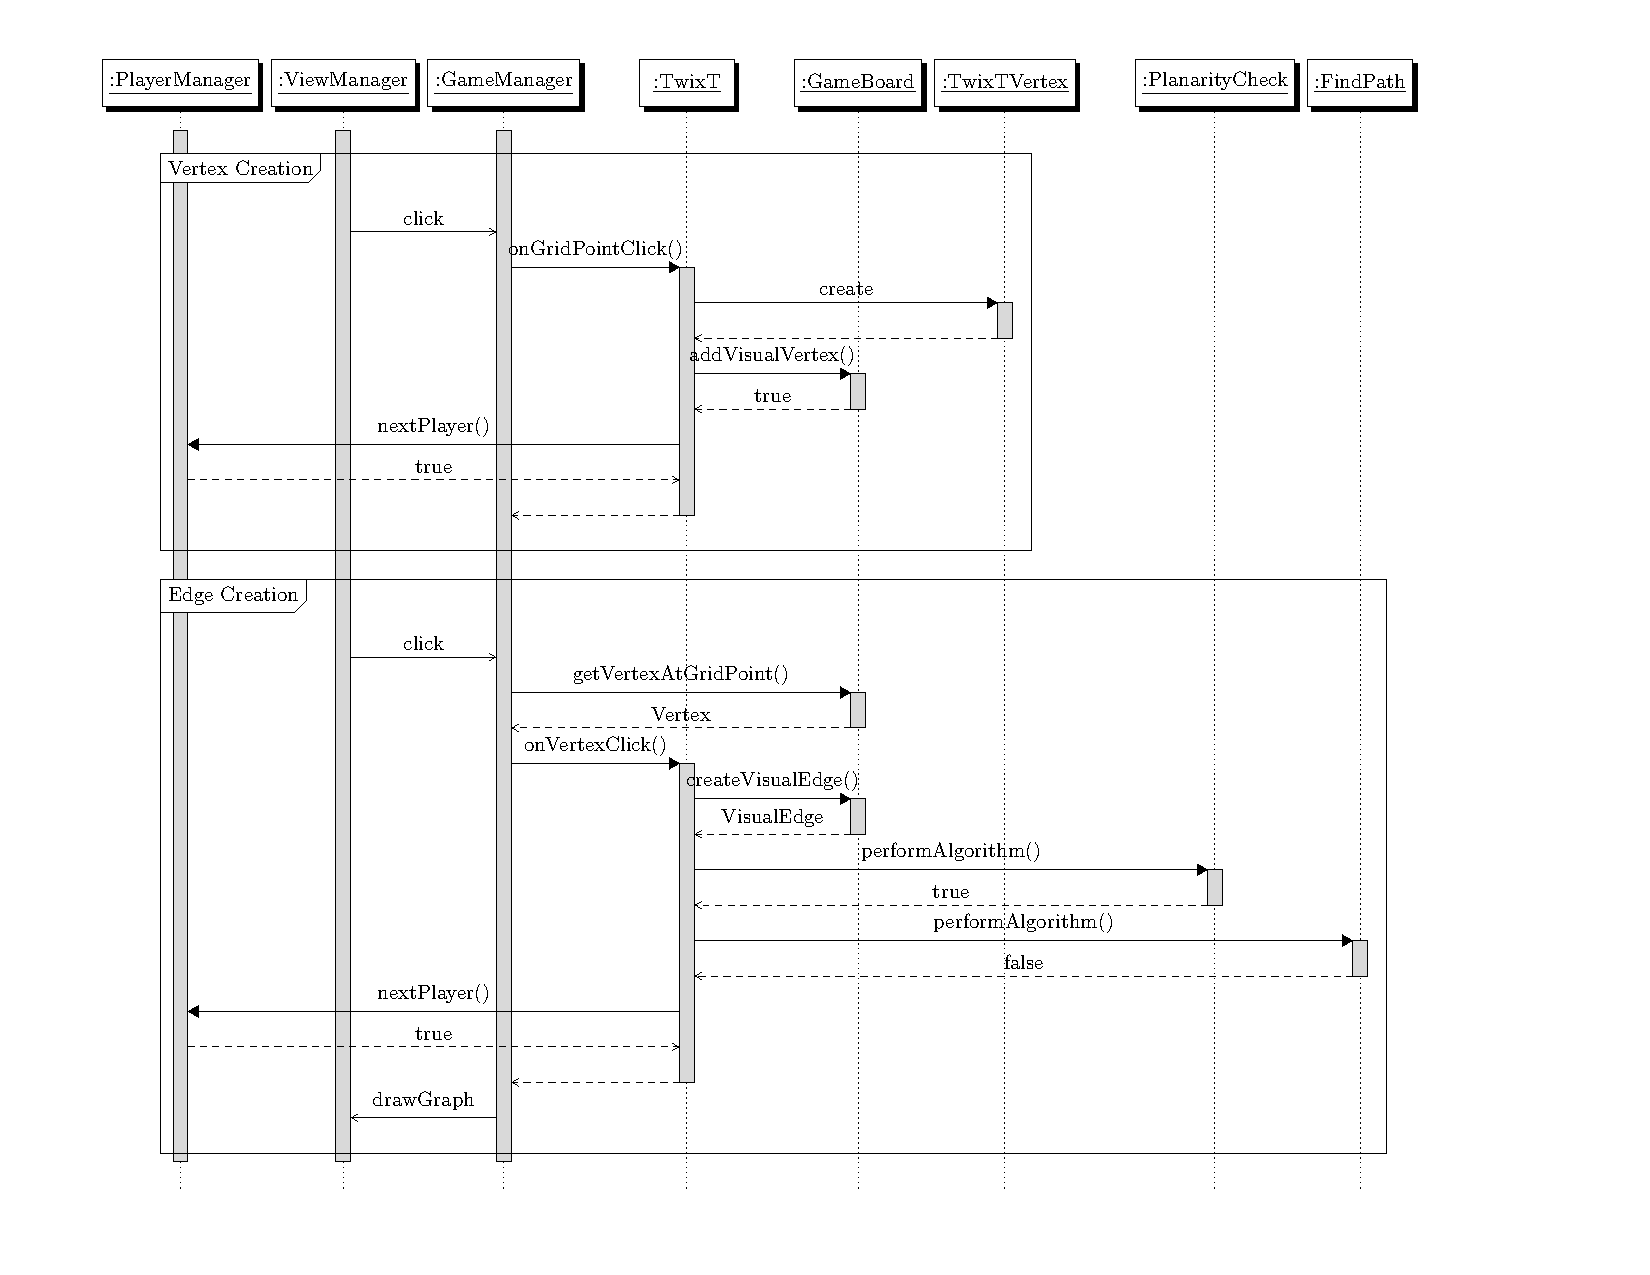
\includegraphics[page=1,angle=90,width=1\textwidth]{seqTwixt.pdf}
	\caption{Sequence diagram showing the process of creating vertices and edges in the game implementation \twixt.}
	\label{img:seqTwixt}
\end{figure}

\begin{figure}[h]
	\centering
	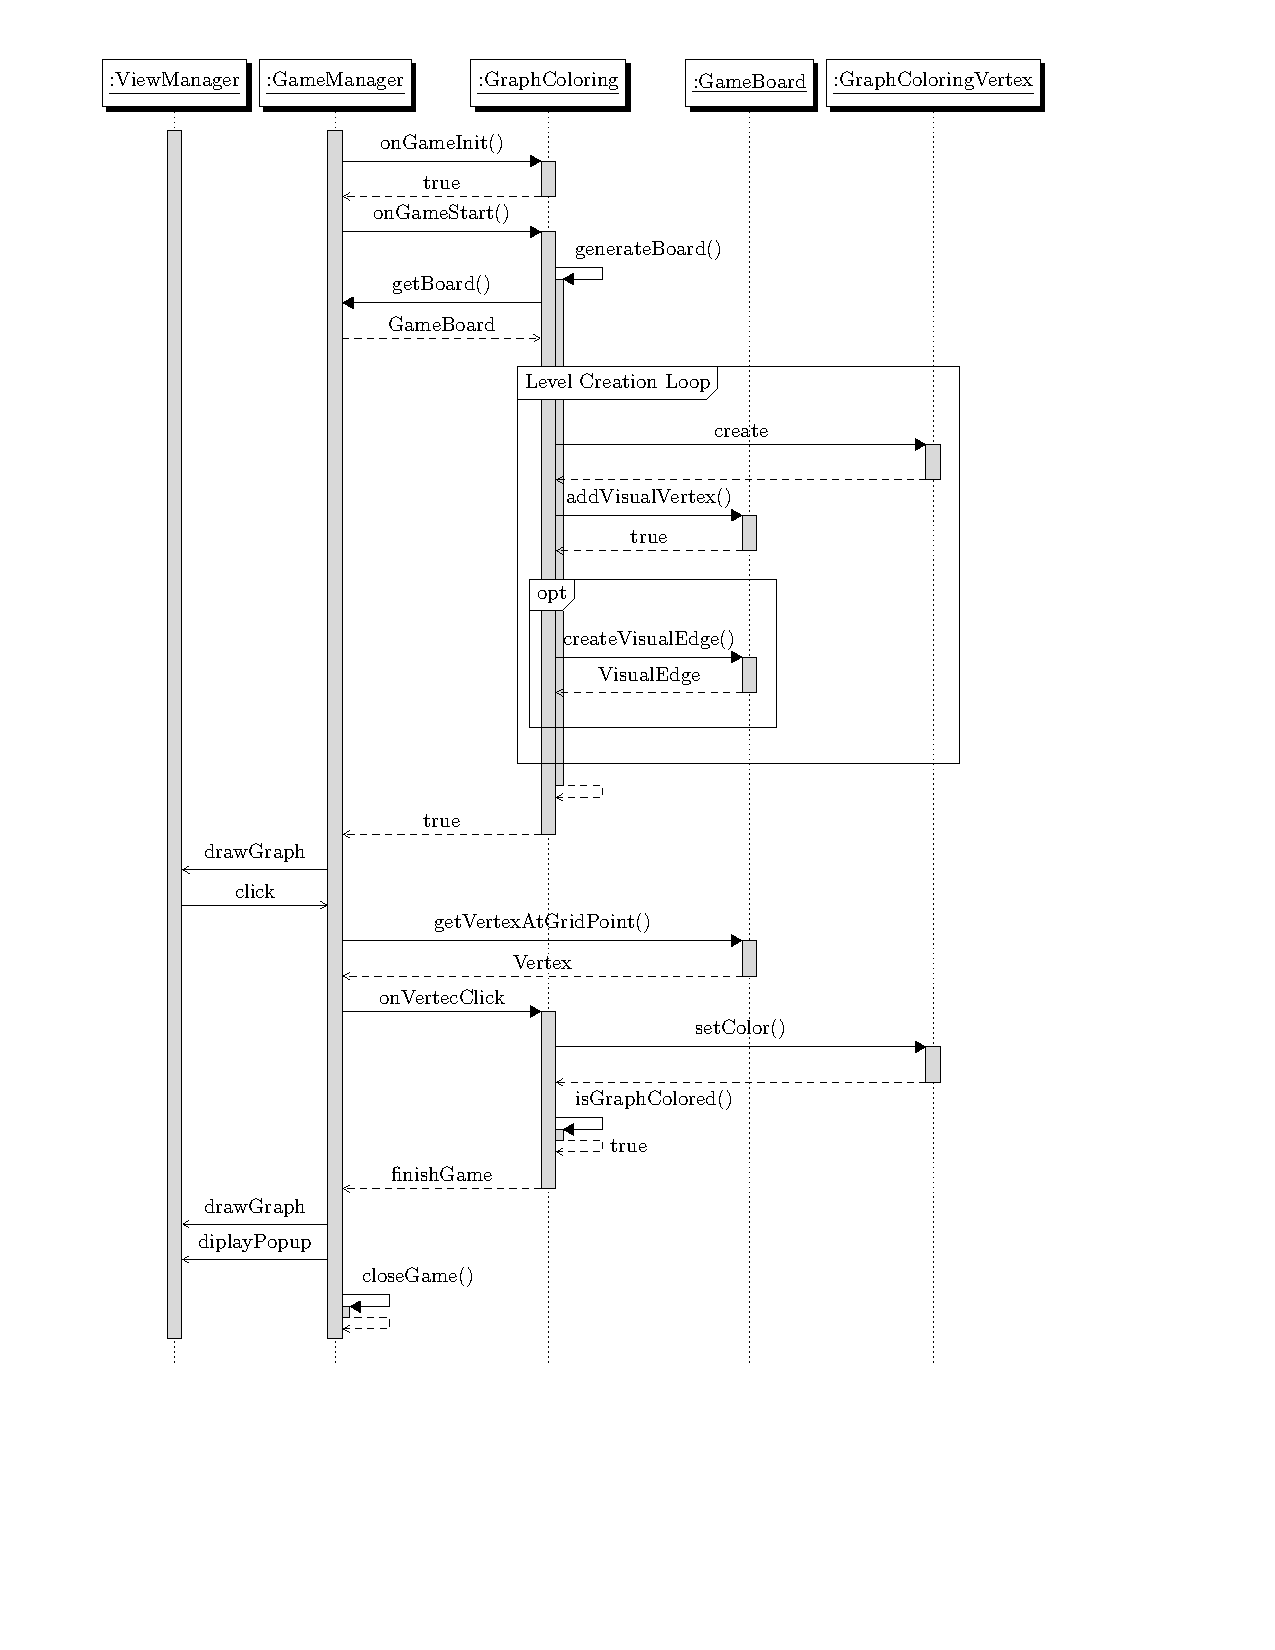
\includegraphics[width=1\textwidth]{seqGraphcoloring.pdf}
	\caption{Sequence diagram showing the process of initializing a new \graphcoloring game.}
	\label{img:seqGraphcoloring}
\end{figure}

\begin{figure}[h]
	\centering
	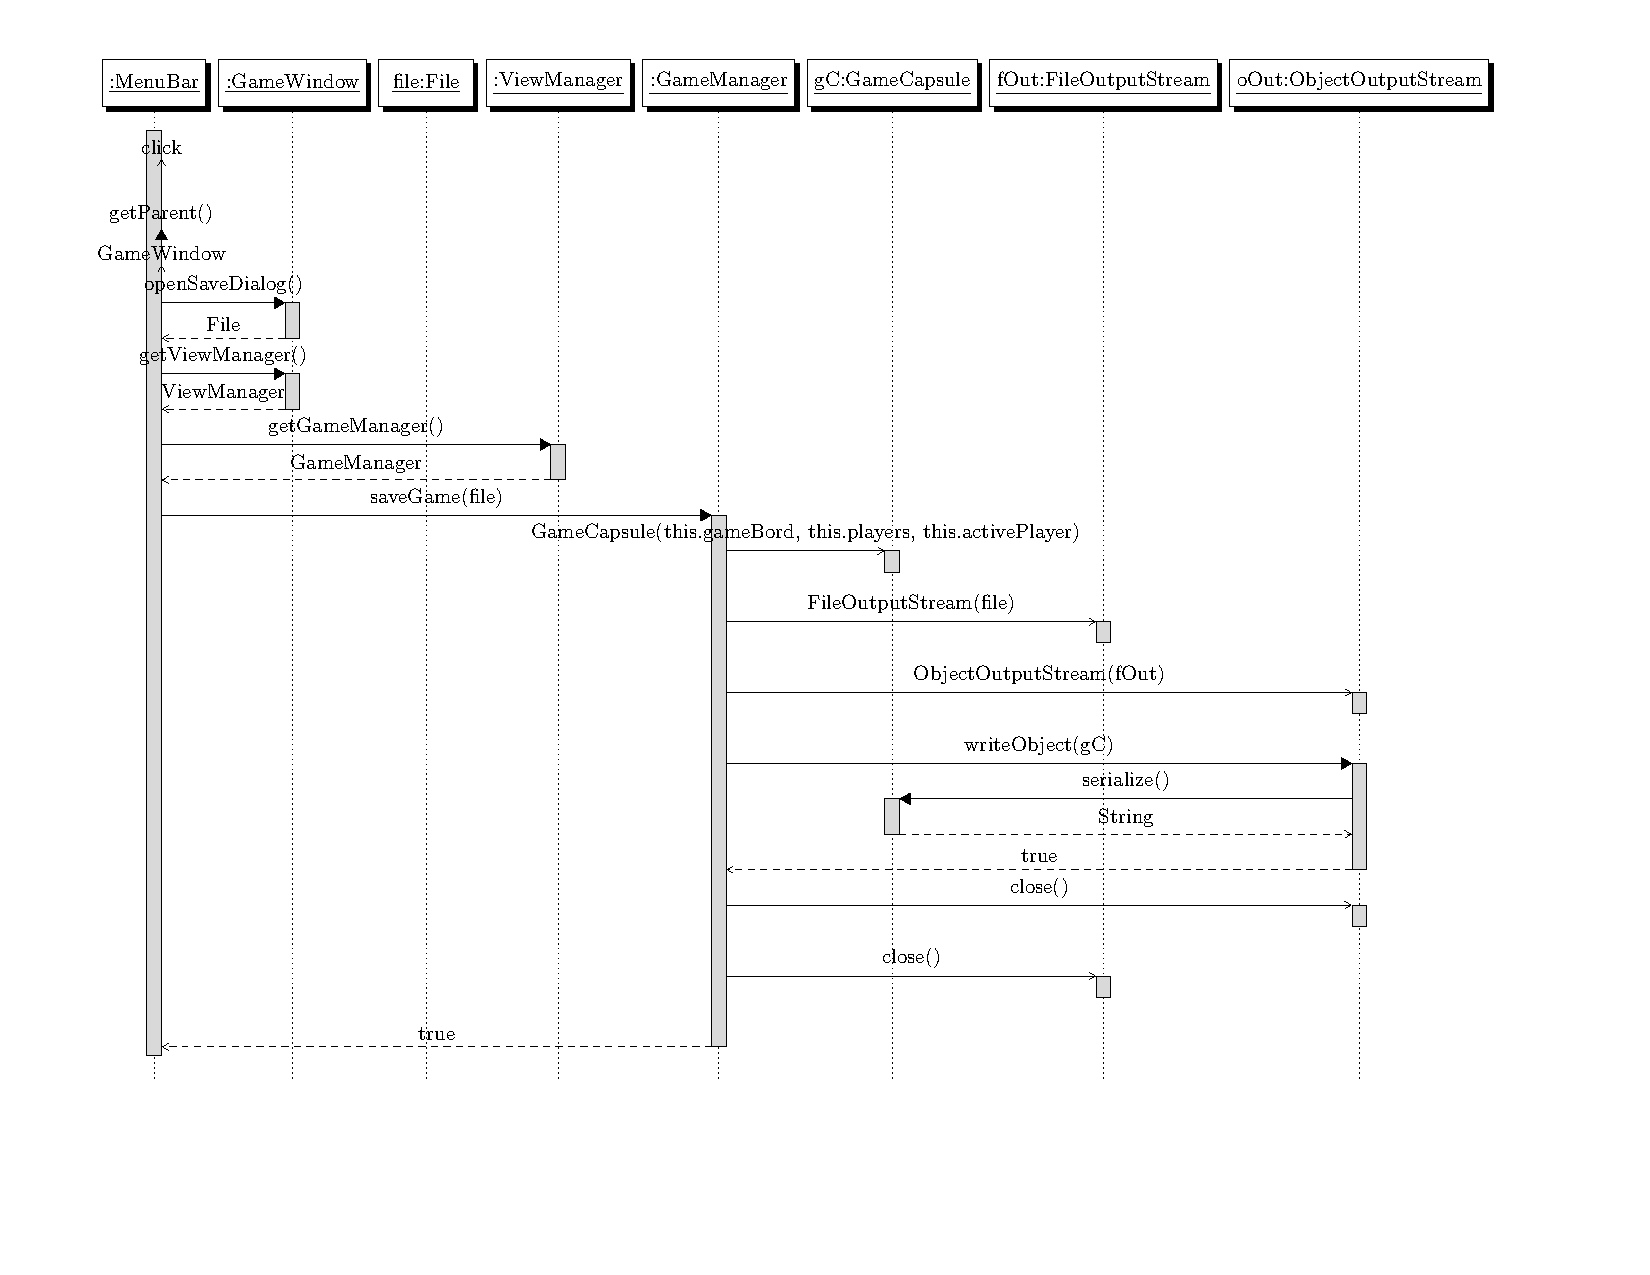
\includegraphics[page=1,angle=90,width=1\textwidth]{seqSaveLoadGame.pdf}
	\caption{Sequence diagram showing the process of saving a game.}
	\label{img:seqSaveLoadGame}
\end{figure}

\begin{figure}[h]
	\centering
	\includegraphics[page=2,angle=90,width=1\textwidth]{seqSaveLoadGame.pdf}
	\caption{Sequence diagram showing the process of loading a game.}
	\label{img:seqSaveLoadGame}
\end{figure}